\subsection{Aplicação Painel: 2ª via código de barras}
\subsubsection*{Descrição do caso de uso}
Caso pretenda, um utilizador do painel também pode re-imprimir um código de barras sem necessidade de abrir a aplicação Fábrica. Para isso o utilizador necessita pressionar o botão 2ª via do código de barras na linha referente ao registo que pretende atualizar. Pelo facto de ser apenas uma procedimento executado em background, não possui nenhuma view.

\subsubsection*{Models compatíveis com o caso de uso}
Este caso de uso é compatível com os models Recolhas, Produto Acabado.

\subsubsection*{Fluxo do caso de uso}
O caso de uso inicia-se quando o utilizador pressionar o botão 2ª via de código de barras da linha do registo. Um novo separador abre-se com o código de barras pronto a ser impresso.


\begin{figure}[H] 
	\begin{center}
		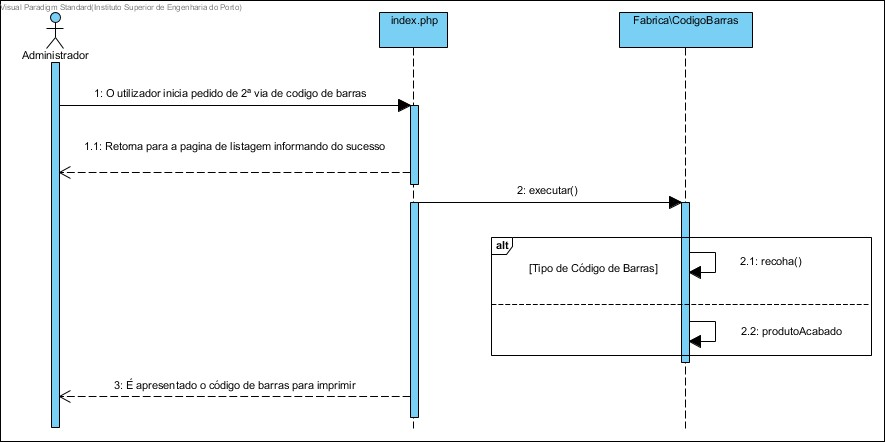
\includegraphics[width=\textwidth,keepaspectratio]{figuras/Diagramas_vp/SD_Painel_6_2_via_Codigo_de_Barras.jpg}
		\caption{Diagrama de sequência imprimir 2ª via do código de barras}
		\label{fig:sd_2_via_painel} 
	\end{center}
\end{figure}